\begin{figure}[t]
  \centering
  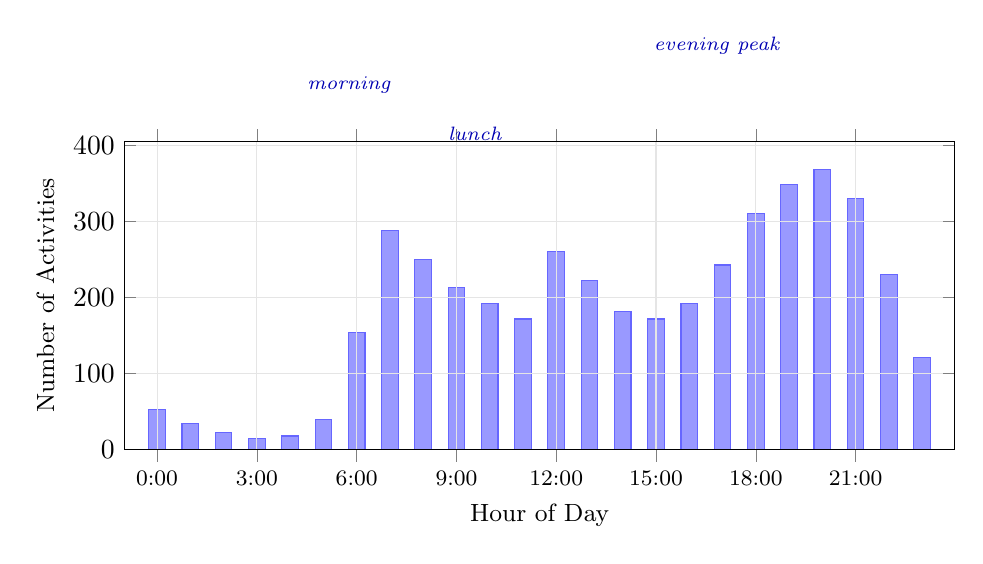
\begin{tikzpicture}
    \begin{axis}[
      width=\columnwidth,
      height=5.5cm,
      ybar,
      bar width=6pt,
      ylabel={Number of Activities},
      ylabel style={font=\small},
      xlabel={Hour of Day},
      xlabel style={font=\small},
      xmin=-0.5, xmax=23.5,
      ymin=0,
      xtick={0,3,6,9,12,15,18,21},
      xticklabels={0:00,3:00,6:00,9:00,12:00,15:00,18:00,21:00},
      x tick label style={font=\footnotesize},
      grid=major,
      grid style={gray!20},
      enlarge x limits=0.02,
      area style,
    ]
    \addplot[fill=blue!40, draw=blue!60] coordinates {
      (0,53)  (1,35)  (2,23)   (3,15)   (4,18)   (5,40)
      (6,154)  (7,288) (8,250)  (9,213)  (10,192) (11,172)
      (12,261)(13,223) (14,182) (15,172) (16,192) (17,243)
      (18,311)(19,349)(20,369)(21,331)(22,230)  (23,121)
    };
    \end{axis}

    % Annotation arrows
    \begin{scope}
      \node[font=\scriptsize\itshape, text=blue!70!black, anchor=south]
        at (2.85, 4.4) {morning};
      \node[font=\scriptsize\itshape, text=blue!70!black, anchor=south]
        at (4.45, 3.8) {lunch};
      \node[font=\scriptsize\itshape, text=blue!70!black, anchor=south west]
        at (6.6, 4.9) {evening peak};
    \end{scope}
  \end{tikzpicture}
  \caption{Temporal distribution of 4{,}307 LLM-generated activities
  across 28~scenes (7~simulated days each, GPT-OSS~20B).  The distribution shows
  clear circadian structure with peaks at morning (07:00), lunch
  (12:00), and evening (18:00--21:00), consistent with real-world
  activity datasets.}
  \label{fig:temporal}
\end{figure}
